\documentclass[10pt,a4paper]{article}
\usepackage[margin=2.2cm]{geometry}
\usepackage[T1]{fontenc}
\usepackage[utf8]{inputenc}
\usepackage{lmodern}
\usepackage{microtype}
\usepackage{graphicx}
\usepackage{booktabs}
\usepackage{tabularx}
\usepackage{siunitx}
\usepackage{amsmath,amssymb}
\usepackage{xcolor}
\usepackage{subcaption}
\usepackage{enumitem}
\usepackage{longtable}
\usepackage{placeins}
\usepackage{caption}
\usepackage[colorlinks=true,linkcolor=blue!50!black,citecolor=blue!50!black,urlcolor=blue!50!black]{hyperref}
\captionsetup{font=small,labelfont=bf}
\setlist{nosep,leftmargin=1.3em}

% model colours = figure palette (categorical slots 1-3)
\definecolor{mA}{HTML}{2A78D6}
\definecolor{mB}{HTML}{EB6834}
\definecolor{mC}{HTML}{1BAF7A}
\newcommand{\A}{\textcolor{mA}{\textbf{A}}}
\newcommand{\B}{\textcolor{mB}{\textbf{B}}}
\newcommand{\C}{\textcolor{mC}{\textbf{C}}}
\newcommand{\bpbunit}{\,bpb}

\newcommand{\paramsA}{54.5}
\newcommand{\meanbpbA}{1.778}
\newcommand{\bpbAweb}{1.450}
\newcommand{\bpbAcode}{2.423}
\newcommand{\bpbAmath}{1.921}
\newcommand{\bpbAwiki}{1.320}
\newcommand{\bpbAatest}{1.266}
\newcommand{\hellaswagA}{28.4}
\newcommand{\arceasyA}{31.6}
\newcommand{\piqaA}{52.3}
\newcommand{\lambadaA}{11.1}
\newcommand{\lambadapplA}{710}
\newcommand{\tputA}{142}
\newcommand{\decodeA}{6.6}
\newcommand{\vramA}{0.58}
\newcommand{\tokensA}{0.38}
\newcommand{\flopsA}{1.25\times10^{17}}
\newcommand{\kwhpreA}{0.09}
\newcommand{\kwhtotA}{0.1}
\newcommand{\hoursA}{7.1}
\newcommand{\tppA}{7}
\newcommand{\paramsB}{100.7}
\newcommand{\meanbpbB}{1.052}
\newcommand{\bpbBweb}{1.109}
\newcommand{\bpbBcode}{0.755}
\newcommand{\bpbBmath}{1.219}
\newcommand{\bpbBwiki}{1.123}
\newcommand{\bpbBatest}{1.438}
\newcommand{\hellaswagB}{33.6}
\newcommand{\arceasyB}{47.7}
\newcommand{\piqaB}{61.6}
\newcommand{\lambadaB}{24.5}
\newcommand{\lambadapplB}{22}
\newcommand{\tputB}{66}
\newcommand{\decodeB}{15.0}
\newcommand{\vramB}{0.86}
\newcommand{\tokensB}{3.42}
\newcommand{\flopsB}{2.26\times10^{18}}
\newcommand{\kwhpreB}{7.93}
\newcommand{\kwhtotB}{10.5}
\newcommand{\hoursB}{15.7}
\newcommand{\tppB}{34}
\newcommand{\meanbpblongB}{0.979}
\newcommand{\paramsC}{343.7}
\newcommand{\meanbpbC}{0.991}
\newcommand{\bpbCweb}{1.071}
\newcommand{\bpbCcode}{0.721}
\newcommand{\bpbCmath}{1.096}
\newcommand{\bpbCwiki}{1.075}
\newcommand{\bpbCatest}{1.326}
\newcommand{\hellaswagC}{35.7}
\newcommand{\arceasyC}{56.0}
\newcommand{\piqaC}{66.6}
\newcommand{\lambadaC}{32.9}
\newcommand{\lambadapplC}{11}
\newcommand{\tputC}{27}
\newcommand{\decodeC}{31.2}
\newcommand{\vramC}{2.21}
\newcommand{\tokensC}{5.46}
\newcommand{\flopsC}{1.22\times10^{19}}
\newcommand{\kwhpreC}{51.10}
\newcommand{\kwhtotC}{99.5}
\newcommand{\hoursC}{101.3}
\newcommand{\tppC}{16}
\newcommand{\meanbpblongC}{0.921}
\newcommand{\nonpadA}{39}
\newcommand{\uniqueA}{37}
\newcommand{\benchN}{2000}

\newcommand{\hsgptTwo}{34.8}
\newcommand{\lambgptTwo}{34.5}
\newcommand{\arcgptTwo}{44.5}
\newcommand{\piqagptTwo}{62.2}
\newcommand{\bpbgptTwo}{1.243}
\newcommand{\hsgptTwoMed}{38.6}
\newcommand{\lambgptTwoMed}{44.1}
\newcommand{\arcgptTwoMed}{49.4}
\newcommand{\piqagptTwoMed}{67.3}
\newcommand{\bpbgptTwoMed}{1.107}
\newcommand{\hspythiaS}{33.7}
\newcommand{\lambpythiaS}{34.8}
\newcommand{\arcpythiaS}{44.3}
\newcommand{\piqapythiaS}{61.8}
\newcommand{\bpbpythiaS}{1.024}
\newcommand{\hspythiaM}{38.2}
\newcommand{\lambpythiaM}{51.2}
\newcommand{\arcpythiaM}{52.8}
\newcommand{\piqapythiaM}{68.2}
\newcommand{\bpbpythiaM}{0.885}
\newcommand{\hsoptS}{34.5}
\newcommand{\lamboptS}{39.4}
\newcommand{\arcoptS}{43.2}
\newcommand{\piqaoptS}{61.8}
\newcommand{\bpboptS}{1.194}
\newcommand{\hssmolS}{38.9}
\newcommand{\lambsmolS}{43.8}
\newcommand{\arcsmolS}{64.3}
\newcommand{\piqasmolS}{68.6}
\newcommand{\bpbsmolS}{0.895}
\newcommand{\hssmolM}{43.5}
\newcommand{\lambsmolM}{54.4}
\newcommand{\arcsmolM}{70.3}
\newcommand{\piqasmolM}{72.7}
\newcommand{\bpbsmolM}{0.796}
\newcommand{\flopsratioCgptS}{18}
\newcommand{\tokratioCgptS}{55}


\title{\textbf{Three Small Language Models, One Yardstick}\\[2pt]
\large A uniform evaluation of checkpoints \A{}, \B{} and \C{}, with GPT-3 and open baselines}
\author{Model comparison report}
\date{November 2026}

\begin{document}
\maketitle

\begin{abstract}
\noindent We compare three decoder-only Transformer language models trained from scratch on a workstation with two RTX~2070~Super GPUs:
\A{}, a \paramsA\,M-parameter GPT-2-style model pre-trained on a small mixed-domain corpus;
\B{}, a \paramsB\,M-parameter Llama-style model taken through pre-training, mid-training and a full post-training pipeline (SFT, DPO, GRPO, self-distillation); and
\C{}, a \paramsC\,M-parameter model of the same family, put through the same pipeline at larger scale.
Because the models use three different tokenizers, we score language-modelling quality in \emph{bits per byte} of identical raw text, and we run every model through the same zero-shot benchmark harness.
\C{} is the best model on every quality metric except A's own lower-cased test set: mean \meanbpbC\bpbunit{} against \meanbpbB{} for \B{} and \meanbpbA{} for \A{}, and HellaSwag \hellaswagC\% against \hellaswagB\% and \hellaswagA\%.
\B{} gets about 92\% of \C{}'s bpb gain over \A{} with less than a third of its parameters and about a fifth of its pre-training compute.
Compared with the original GPT-3 family, \C{} matches or beats GPT-3 Small on three of four zero-shot tasks with about 1/18 of its training compute. Against open models of similar size (GPT-2, OPT, Pythia, SmolLM2) measured with the same harness, B and C are competitive per FLOP but trail the models trained on far more tokens. \A{} is the cheapest model by one to two orders of magnitude, but it is barely above chance on reasoning benchmarks, cannot model case or code well, and is limited to a 512-token context.
\end{abstract}

\section{Models under test}

\begin{table}[h]
\centering\small
\begin{tabularx}{\linewidth}{l>{\raggedright}X>{\raggedright}X>{\raggedright\arraybackslash}X}
\toprule
 & \A{} & \B{} & \C{} \\
\midrule
Checkpoint & \texttt{a.pt}, step 60\,000 (epoch 10) & \texttt{b.pt}, final post-trained model & \texttt{c.pt}, final post-trained model \\
Lineage & \texttt{QPT-LLM-prototype-no-lib} & \texttt{llm\_pipeline/work} (``100M'' run) & \texttt{llm\_pipeline/work\_350m} \\
Layers / $d_\text{model}$ / heads & 12 / 512 / 8 (MHA) & 12 / 768 / 12 (4 KV heads, GQA) & 28 / 1024 / 16 (4 KV heads, GQA) \\
Block & pre-norm LayerNorm, GELU MLP ($4d$), biases & pre-norm RMSNorm, SwiGLU ($d_\text{ff}{=}2048$) & pre-norm RMSNorm, SwiGLU ($d_\text{ff}{=}2752$) \\
Positions & learned absolute, 512 max & RoPE + YaRN-style scaling, 4096 & RoPE + YaRN-style scaling, 4096 \\
Unique parameters & \paramsA\,M (tied emb.) & \paramsB\,M (tied emb.) & \paramsC\,M (tied emb.) \\
Tokenizer & BPE 32k, \emph{lower-cases and strips accents} & byte-level BPE 32\,768 & byte-level BPE 32\,768 (separate training) \\
Pre-training data & 9 HF corpora (news, reviews, Wikipedia, Q\&A); \uniqueA\,M unique tokens, 10 epochs & web 74\%, code 12\%, math 8\%, wiki 6\% & same mix, about 2.3$\times$ more text \\
Tokens seen (pre-train) & \tokensA\,B & \tokensB\,B & \tokensC\,B \\
Tokens per parameter & \tppA & \tppB & \tppC \\
Post-training & none (base LM) & mid-train $\to$ SFT $\to$ RM $\to$ DPO $\to$ GRPO $\to$ distill & same \\
\bottomrule
\end{tabularx}
\caption{The three checkpoints. Parameter counts are unique tensors (the tied input/output embedding is counted once).}
\label{tab:models}
\end{table}

\paragraph{Provenance note.}
The \texttt{tokens\_c/} directory shipped next to \texttt{c.pt} holds the tokenizer of the pipeline's \emph{smoke-test} run, with a vocabulary of 4\,096 (its MD5 hash matches \texttt{work\_smoke}). It cannot encode text for \C{}, whose embedding table has 32\,768 rows. All results for \C{} therefore use the tokenizer of the run that produced it, \texttt{work\_350m/3\_tokenization/tokenizer.json}. \texttt{a.pt} matches A's training checkpoint \texttt{ckpt\_step\_0060000.pt} byte for byte.

\section{Methodology}

\paragraph{Tokenizer-independent perplexity.}
Per-token loss cannot be compared across different vocabularies, so we report bits per byte:
\[
\text{bpb}=\frac{\sum_t -\ln p(x_t\mid x_{<t})}{\ln 2\cdot N_\text{bytes}},
\]
where $N_\text{bytes}$ is the UTF-8 length of the \emph{original} text.
Each model re-tokenizes the same documents with its own tokenizer. Every document is scored on its own, starting from BOS, in non-overlapping windows of 512 tokens (A's maximum context). B and C are also scored with 2\,048-token windows.
The text comes from five held-out sets of about 0.55--0.67\,MB each:
the web, code, math and Wikipedia validation shards of the B pipeline, and A's own test split (``A-test'', which was lower-cased by A's preprocessing).

\emph{Check:} A scores 3.954 nats/token on A-test with this harness, against 3.957 in its training log, so the reimplementation of A is faithful.
We found that A was trained on single documents padded to 512 tokens (only \nonpadA\% of its training tokens are real text). Scoring it on packed multi-document windows would therefore be unfair to it, and that is why every document is scored on its own.

\paragraph{Zero-shot benchmarks.}
HellaSwag, ARC-Easy and PIQA are scored by the log-likelihood of each answer, using the pipeline's own harness logic (\texttt{eval/benchmarks.py}). We report length-normalised accuracy (acc\_norm) for HellaSwag and PIQA and raw accuracy for ARC-Easy. LAMBADA requires an exact greedy prediction of the final word. Each benchmark uses the first \benchN{} items, or 1\,838 for PIQA, and the error bars are 95\% Wilson intervals.
All three models are run on the same items with the same prompts. A's inputs are left-truncated to 512 tokens.

\paragraph{Efficiency.}
We measure fp16 forward throughput at sequence length 512 (batch sizes 1 and 8), greedy decode latency without a KV cache (identical for all models), peak allocated VRAM, and checkpoint size, all on one RTX~2070~Super.
Training compute, energy and wall-clock time come from the training logs. For A, compute is estimated as $6ND$ over non-pad tokens.

\section{Results}

\subsection{Language-modelling quality}

\begin{figure}[h]
\centering
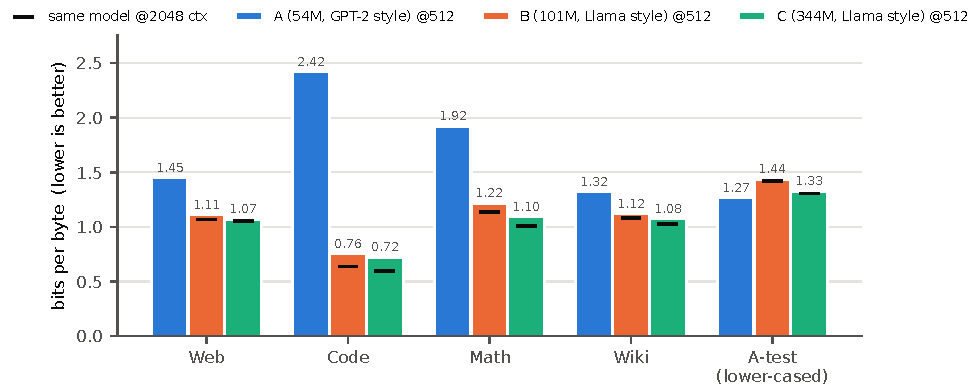
\includegraphics[width=\linewidth]{figs/bpb_domains.pdf}
\caption{Bits per byte on identical raw text, using 512-token windows (bars). Black ticks show B and C with 2\,048-token windows. Lower is better.}
\label{fig:bpb}
\end{figure}

\begin{table}[h]
\centering\small
\begin{tabular}{lrrrrr}
\toprule
Model / context & Web & Code & Math & Wiki & A-test \\
\midrule
A @ 512 & 1.450 & 2.423 & 1.921 & 1.320 & 1.266 \\
B @ 512 & 1.109 & 0.755 & 1.219 & 1.123 & 1.438 \\
B @ 2048 & 1.068 & 0.637 & 1.133 & 1.079 & 1.419 \\
C @ 512 & 1.071 & 0.721 & 1.096 & 1.075 & 1.326 \\
C @ 2048 & 1.054 & 0.595 & 1.004 & 1.030 & 1.305 \\
\midrule
A bytes/token & 4.62 & 3.05 & 3.47 & 4.38 & 4.50 \\
B bytes/token & 4.41 & 3.81 & 3.56 & 3.89 & 4.01 \\
C bytes/token & 4.40 & 3.79 & 3.56 & 3.88 & 4.01 \\
\bottomrule
\end{tabular}

\caption{Bits per byte by domain and context length. The bottom block shows tokenizer compression (bytes per token, higher means fewer tokens for the same text).}
\label{tab:bpb}
\end{table}

\noindent Figure~\ref{fig:bpb} and Table~\ref{tab:bpb} show four patterns:
\begin{itemize}
  \item \textbf{Size and data order the models consistently.} \C{} $<$ \B{} $<$ \A{} on all four pipeline domains. The mean over the four pipeline domains is \meanbpbC{}, \meanbpbB{} and \meanbpbA\bpbunit{}.
  \item \textbf{A's biggest gap is code} (\bpbAcode{} vs.\ \bpbCcode\bpbunit). Its corpus has essentially no source code, and its normaliser lower-cases identifiers and strips accents, so its tokenizer fragments code into short pieces (about 3 bytes/token, against 3.8 for B and C).
  \item \textbf{A-test is A's home ground, and A wins there.} The text is already lower-cased and comes from A's own distribution. \A{} scores \bpbAatest{}, ahead of \C{} (\bpbCatest) and \B{} (\bpbBatest). On in-distribution text, a small model trained on that data beats much larger general-purpose models.
  \item \textbf{Long context helps B and C.} Scoring with 2\,048-token windows lowers mean bpb to \meanbpblongB{} (B) and \meanbpblongC{} (C). The largest gains are on code and math, where long-range structure matters. A cannot use context beyond 512 tokens at all.
\end{itemize}

\subsection{Zero-shot benchmarks}

\begin{figure}[h]
\centering
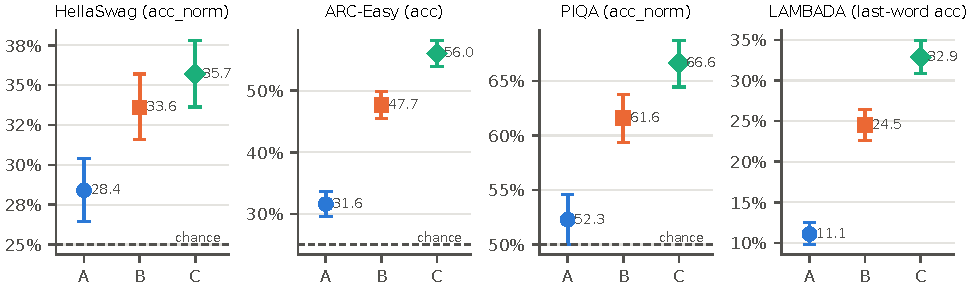
\includegraphics[width=\linewidth]{figs/benchmarks.pdf}
\caption{Zero-shot accuracy with 95\% Wilson intervals. Dashed lines mark chance.}
\label{fig:bench}
\end{figure}

On the benchmarks (Figure~\ref{fig:bench}), \A{} sits a few points above chance on HellaSwag (\hellaswagA\%) and ARC-Easy (\arceasyA\%), and it is barely above chance on PIQA (\piqaA\%, with the interval's lower edge at about 50\%).
\C{} is clearly ahead on ARC-Easy (\arceasyC\%) and PIQA (\piqaC\%), and leads strongly on LAMBADA (\lambadaC\% against \lambadaB\% and \lambadaA\%). LAMBADA tests long-range narrative tracking, which is exactly where depth and data help.
On HellaSwag, \B{} (\hellaswagB\%) and \C{} (\hellaswagC\%) are close. At this scale HellaSwag rises slowly, as Figure~\ref{fig:curves} (right) shows.
LAMBADA perplexity separates the models most sharply: \lambadapplA{} for A, \lambadapplB{} for B and \lambadapplC{} for C.

\subsection{Training dynamics, data and compute}

\begin{figure}[h]
\centering
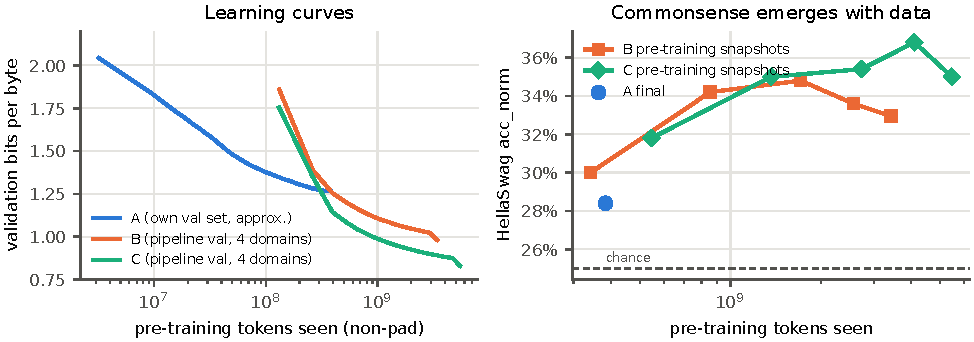
\includegraphics[width=\linewidth]{figs/curves.pdf}
\caption{Left: validation bpb during pre-training, read from the logs. B and C were evaluated on the pipeline's 4-domain validation set. A's curve is its own validation loss converted to bpb using its measured 4.48 bytes/token, so it is approximate and on a different text distribution. Right: HellaSwag accuracy of B and C at pre-training snapshots (10\%, 25\%, 50\%, 75\%, 100\%), with A's final checkpoint for reference.}
\label{fig:curves}
\end{figure}

\begin{figure}[h]
\centering
\begin{minipage}{0.36\linewidth}\centering
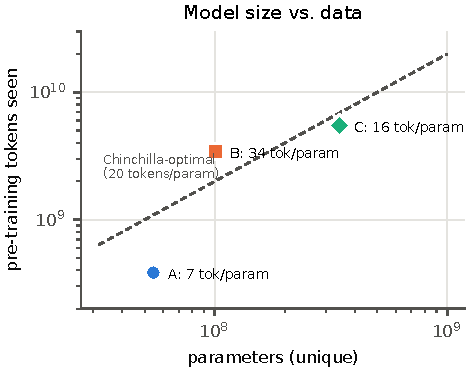
\includegraphics[width=\linewidth]{figs/data_scale.pdf}
\end{minipage}\hfill
\begin{minipage}{0.62\linewidth}\centering
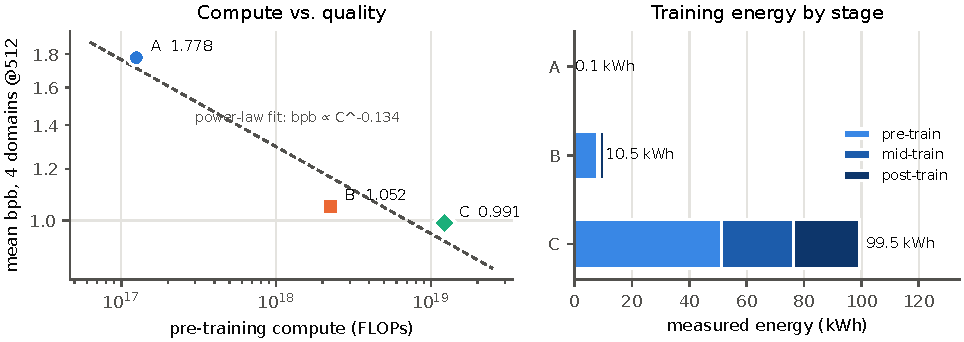
\includegraphics[width=\linewidth]{figs/scaling_energy.pdf}
\end{minipage}
\caption{Left: parameters vs.\ pre-training tokens. A saw only \tppA{} tokens per parameter, cycling 10 times over \uniqueA\,M unique tokens. B was trained past the Chinchilla ratio, and C sits just below it. Centre: pre-training compute vs.\ uniform mean bpb, with a power-law fit through the three points. Right: measured training energy by stage.}
\label{fig:scaling}
\end{figure}

Figure~\ref{fig:scaling} gives the economics:
\begin{itemize}
  \item \textbf{Compute.} Pre-training cost about $\flopsA$ FLOPs for A, $\flopsB$ for B and $\flopsC$ for C.
  \item \textbf{Scaling.} Mean bpb falls roughly as a power law in compute. A, though, is off the B--C trend: its architecture is older, its corpus is narrow and lower-cased, and it repeated the same 37\,M tokens ten times.
  \item \textbf{Energy.} Measured end-to-end training energy, from pre-training through post-training, is \kwhtotA{} kWh for A, \kwhtotB{} kWh for B and \kwhtotC{} kWh for C. C's mid-training and full-length SFT cost almost as much energy as its pre-training.
  \item \textbf{Caveat on A's energy.} A's figure is the prototype's own GPU-side meter over \hoursA{} h. It is not directly comparable with the pipeline's whole-system estimate, and likely understates A's true energy.
\end{itemize}

\subsection{Inference efficiency}

\begin{figure}[h]
\centering
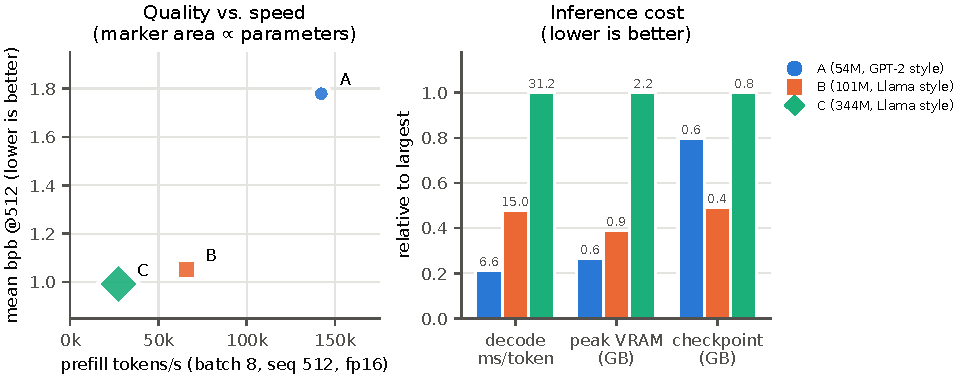
\includegraphics[width=\linewidth]{figs/efficiency.pdf}
\caption{Left: quality vs.\ prefill throughput. Right: inference cost, normalised to the most expensive model, with absolute values printed above the bars.}
\label{fig:eff}
\end{figure}

A processes about \tputA{}k tokens/s at batch 8, against \tputB{}k for B and \tputC{}k for C. Its greedy decode takes \decodeA{} ms/token, against \decodeB{} and \decodeC{} ms, and it fits in \vramA{} GB, against \vramB{} and \vramC{} GB (Figure~\ref{fig:eff}).
\B{} sits at the knee of the curve. It is about 2.4$\times$ faster than \C{} and costs only about \(\meanbpbB-\meanbpbC\) bpb.

\subsection{Inside the networks}

\begin{figure}[h]
\centering
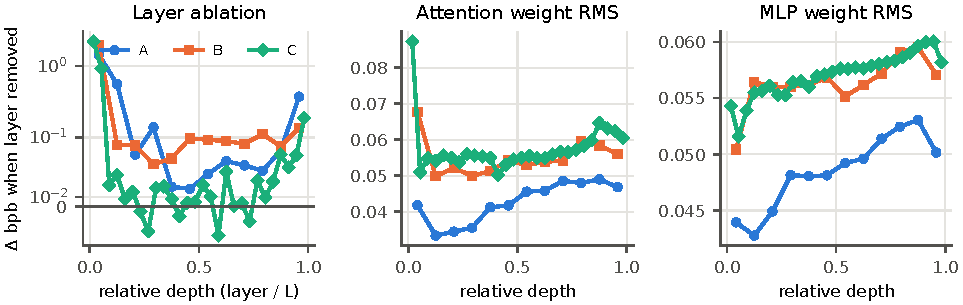
\includegraphics[width=\linewidth]{figs/layers.pdf}
\caption{Left: increase in bpb when one whole block is skipped (web + wiki text, symmetric log scale). Middle and right: RMS of each block's attention and MLP weights, plotted against relative depth.}
\label{fig:layers}
\end{figure}

All three models depend most on their first block: skipping it costs 1.4--2.2 bpb (Figure~\ref{fig:layers}).
\begin{itemize}
  \item \textbf{A and C} also depend heavily on block 1 and on the last block.
  \item \textbf{B} spreads its computation more evenly, at about 0.05--0.14 bpb per block.
  \item \textbf{C's middle layers are redundant.} Many of them cost less than 0.03 bpb when removed, and a few slightly \emph{improve} bpb, making C a natural candidate for depth pruning or early exit.
  \item \textbf{Weight scales differ by family.} The Llama-style models keep their weights roughly flat across depth, apart from a larger first block, consistent with weight decay 0.1 and scaled residual initialisation. A's weights grow steadily with depth.
\end{itemize}

\subsection{What post-training and mid-training bought (B and C)}

\begin{figure}[h]
\centering
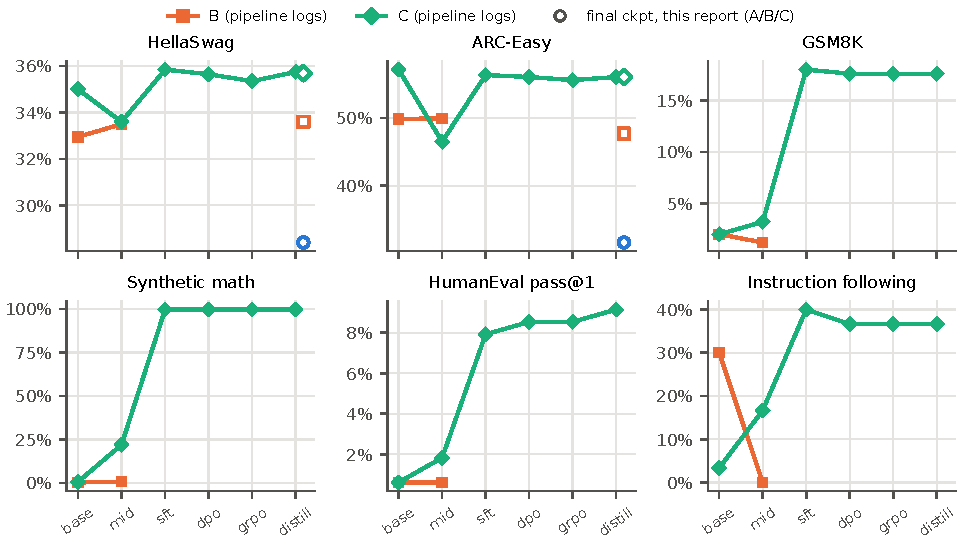
\includegraphics[width=\linewidth]{figs/stages.pdf}
\caption{Capability across pipeline stages, from the pipeline's own evaluation logs. Only base and mid-training were evaluated for B. Hollow markers show the final checkpoints measured in this report, on the same items.}
\label{fig:stages}
\end{figure}

\begin{figure}[h]
\centering
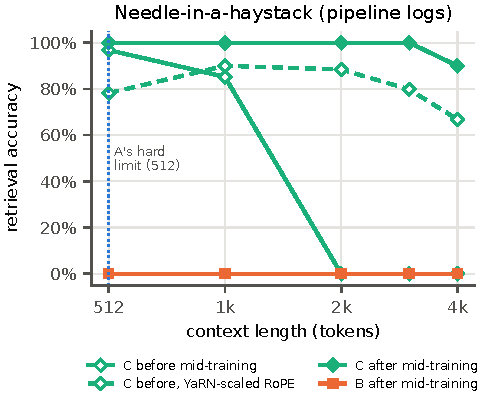
\includegraphics[width=0.5\linewidth]{figs/needle.pdf}
\caption{Needle-in-a-haystack retrieval, from the pipeline logs. Mid-training at 1k$\to$4k tokens with rescaled RoPE gave C near-perfect retrieval up to 4\,096 tokens. B never retrieved the needle.}
\label{fig:needle}
\end{figure}

The pipeline logs (Figures~\ref{fig:stages}--\ref{fig:needle}) show that post-training transformed what \C{} can do:
\begin{itemize}
  \item \textbf{Math.} Synthetic arithmetic accuracy went from about 1\% to 99.6\%, and GSM8K from 2\% to 17.6\%.
  \item \textbf{Code.} HumanEval pass@1 went from 0.6\% to 9.1\%.
  \item \textbf{Long context.} Needle retrieval went from failing beyond 1k tokens to about 90--100\% up to 4k.
  \item \textbf{Conversation.} Multi-turn fact recall reached about 70\% after distillation.
\end{itemize}
The cost was a small rise in raw-text bpb: the pipeline's own log reports 0.82 at the base checkpoint and 0.92 after SFT, a known effect of instruction tuning.
\B{}'s pipeline did not evaluate its post-trained stages, so the hollow markers are its only post-training measurement. A has no instruction or chat ability.

\subsection{Qualitative samples}

Table~\ref{tab:samples} lists greedy continuations.
\begin{itemize}
  \item \textbf{A} produces fluent, lower-case prose but quickly falls into repetition loops.
  \item \textbf{B and C} follow the chat template.
  \item \textbf{B and C} both solve the arithmetic chat prompt ($12\times7=84$), but only \textbf{C} gives a coherent explanation of why the sky is blue. B loops on the wording of the question.
  \item \textbf{Base-mode facts} are shaky for all three: only B and C complete ``The capital of France is'' with Paris, and only C gets close on the boiling point of water.
\end{itemize}

\section{Comparison with GPT-3 and contemporary small models}
\label{sec:baselines}

To place A, B and C in context, we compare them with two groups:
\begin{itemize}
  \item \textbf{GPT-3} (Brown et al., 2020), the original 2020 model family. Its weights were never released, so we take the zero-shot numbers \emph{published} in the paper's Table~H.1. All GPT-3 sizes were trained on 300\,B tokens with a 2\,048-token context. We checked these numbers against the paper; they were not re-measured.
  \item \textbf{Open models of similar size}, run through \emph{exactly the same harness} as A, B and C: the same raw text for bpb, the same benchmark items, prompts and scoring. These are GPT-2 124M and 355M (2019), OPT-125M (2022, 180\,B tokens), Pythia-160M and 410M (2023, 300\,B tokens on the Pile), and SmolLM2-135M and 360M (2024, 2\,T and 4\,T tokens).
\end{itemize}

\begin{table}[h]
\centering\scriptsize
\setlength{\tabcolsep}{4pt}
\begin{tabular}{llrrrrrrrrr}
\toprule
Model & Year & Params & Train tok. & Ctx & HellaSw. & ARC-E & PIQA & LAMB. acc & LAMB. ppl & bpb \\
\midrule
GPT-3 Small$^\dagger$ & 2020 & 125M & 300B & 2048 & 33.7 & 43.6 & 64.6 & 42.7 & 18.6 & -- \\
GPT-3 Medium$^\dagger$ & 2020 & 356M & 300B & 2048 & 43.6 & 46.5 & 70.2 & 54.3 & 9.1 & -- \\
GPT-3 Large$^\dagger$ & 2020 & 760M & 300B & 2048 & 51.0 & 53.0 & 72.9 & 60.4 & 6.5 & -- \\
GPT-3 XL$^\dagger$ & 2020 & 1,320M & 300B & 2048 & 54.7 & 53.8 & 75.1 & 63.6 & 5.4 & -- \\
GPT-3 175B$^\dagger$ & 2020 & 174,600M & 300B & 2048 & 78.9 & 68.8 & 81.0 & 76.2 & 3.0 & -- \\
\midrule
GPT-2 124M & 2019 & 124M & n/r & 1024 & 34.8 & 44.5 & 62.2 & 34.5 & 15.2 & 1.243 \\
GPT-2 355M & 2019 & 355M & n/r & 1024 & 38.6 & 49.4 & 67.3 & 44.1 & 8.9 & 1.107 \\
OPT 125M & 2022 & 125M & 180B & 2048 & 34.5 & 43.2 & 61.8 & 39.4 & 10.9 & 1.194 \\
Pythia 160M & 2023 & 162M & 300B & 2048 & 33.7 & 44.3 & 61.8 & 34.8 & 12.8 & 1.024 \\
Pythia 410M & 2023 & 405M & 300B & 2048 & 38.2 & 52.8 & 68.2 & 51.2 & 5.5 & 0.885 \\
SmolLM2 135M & 2024 & 135M & 2T & 2048 & 38.9 & 64.3 & 68.6 & 43.8 & 7.8 & 0.895 \\
SmolLM2 360M & 2024 & 362M & 4T & 2048 & 43.5 & 70.3 & 72.7 & 54.4 & 5.0 & 0.796 \\
\midrule
\textbf{\A{}} (this work) & 2026 & 54M & 0.38B & 512 & 28.4 & 31.6 & 52.3 & 11.1 & 709.8 & 1.778 \\
\textbf{\B{}} (this work) & 2026 & 101M & 3B & 4096 & 33.6 & 47.7 & 61.6 & 24.5 & 22.5 & 1.052 \\
\textbf{\C{}} (this work) & 2026 & 344M & 5B & 4096 & 35.7 & 56.0 & 66.6 & 32.9 & 10.6 & 0.991 \\
\bottomrule
\end{tabular}

\caption{Zero-shot comparison. $^\dagger$GPT-3 rows are published values (HellaSwag and PIQA on dev, ARC-Easy and LAMBADA on test, full sets). All other rows were measured here on the same items: the first 2\,000 of HellaSwag (dev), ARC-Easy (test) and LAMBADA-OpenAI, and all 1\,838 PIQA dev items. HellaSwag and PIQA are length-normalised accuracy. ``bpb'' is the mean over the four pipeline domains at 512 tokens. Training-token counts are as reported by each model's authors (n/r = not reported).}
\label{tab:baselines}
\end{table}

\begin{figure}[h]
\centering
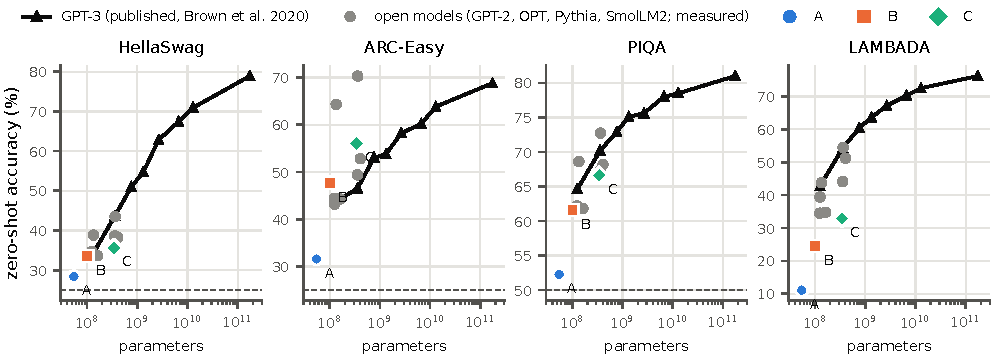
\includegraphics[width=\linewidth]{figs/base_bench_vs_size.pdf}
\caption{Zero-shot accuracy vs.\ parameter count. The black line is the GPT-3 family (published). Grey points are open models measured with our harness. Coloured markers are A, B and C.}
\label{fig:base_size}
\end{figure}

\begin{figure}[h]
\centering
\begin{minipage}{0.38\linewidth}\centering
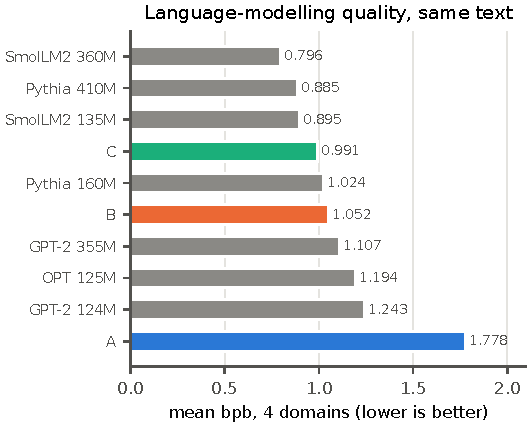
\includegraphics[width=\linewidth]{figs/base_bpb_rank.pdf}
\end{minipage}\hfill
\begin{minipage}{0.6\linewidth}\centering
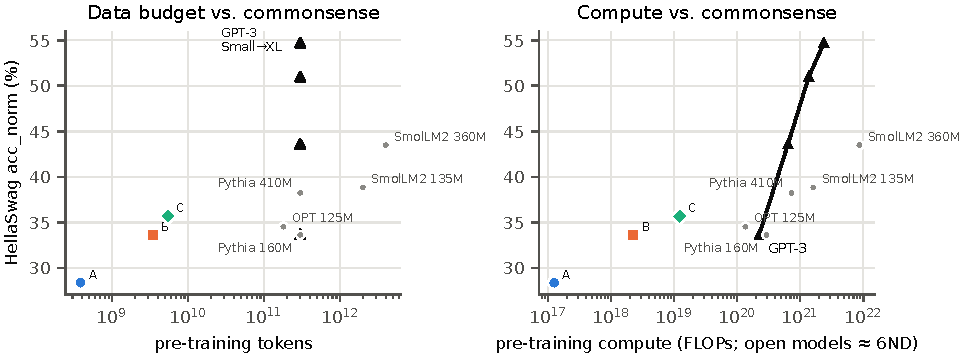
\includegraphics[width=\linewidth]{figs/base_efficiency.pdf}
\end{minipage}
\caption{Left: mean bits per byte on identical text for all ten measured models. Centre and right: HellaSwag against pre-training tokens and against pre-training compute. Compute for open models is estimated as $6ND$; GPT-3 compute is from the paper's Table~D.1.}
\label{fig:base_eff}
\end{figure}

\paragraph{C vs.\ GPT-3.}
\C{} is about the size of GPT-3 Medium (350M) but was trained on \tokratioCgptS$\times$ fewer tokens and with \flopsratioCgptS$\times$ less compute than even GPT-3 \emph{Small}.
\begin{itemize}
  \item \textbf{Against GPT-3 Small (125M),} C matches or beats it on three of four tasks: HellaSwag \hellaswagC{} vs.\ 33.7, ARC-Easy \arceasyC{} vs.\ 43.6, and PIQA \piqaC{} vs.\ 64.6. It falls well short on LAMBADA (\lambadaC{} vs.\ 42.7).
  \item \textbf{Against GPT-3 Medium (350M),} C trails on HellaSwag (43.6), PIQA (70.2) and LAMBADA (54.3), but is ahead on ARC-Easy (46.5).
\end{itemize}
Modern data mixes rich in educational, code and math text explain most of the ARC-Easy gain. The remaining gaps track the 55$\times$ smaller token budget.

\paragraph{A, B, C vs.\ open models of the same size.}
\begin{itemize}
  \item \textbf{B vs.\ GPT-2 124M} (which it slightly undercuts in size): B has better bpb (\meanbpbB{} vs.\ \bpbgptTwo) and ARC-Easy (\arceasyB{} vs.\ \arcgptTwo), similar PIQA (\piqaB{} vs.\ \piqagptTwo), but lower HellaSwag (\hellaswagB{} vs.\ \hsgptTwo) and LAMBADA (\lambadaB{} vs.\ \lambgptTwo).
  \item \textbf{C vs.\ GPT-2 355M,} the closest 2019 model in size: C has better bpb (\meanbpbC{} vs.\ \bpbgptTwoMed) and ARC-Easy (\arceasyC{} vs.\ \arcgptTwoMed), and is behind on HellaSwag (\hellaswagC{} vs.\ \hsgptTwoMed) and LAMBADA (\lambadaC{} vs.\ \lambgptTwoMed).
  \item \textbf{Pythia-410M and SmolLM2-360M,} trained on 55--730$\times$ more tokens than C, are ahead of C on every metric except Pythia's ARC-Easy. SmolLM2-360M is the strongest model measured: bpb \bpbsmolM, HellaSwag \hssmolM, ARC-Easy \arcsmolM, LAMBADA \lambsmolM. Even SmolLM2-135M, at under half of C's size, beats C on every metric (bpb \bpbsmolS, HellaSwag \hssmolS, ARC-Easy \arcsmolS).
  \item \textbf{A} is below every open model on every metric. The smallest of them, OPT-125M, still has more than twice A's parameters and was trained on almost 500$\times$ more tokens.
\end{itemize}

\paragraph{What this means.}
Figure~\ref{fig:base_eff} shows that, at this scale, \emph{training tokens} matter more than architecture:
\begin{itemize}
  \item Among models of comparable size, quality follows the data budget: A (0.4\,B) $<$ B (3.4\,B) $<$ C (5.5\,B) $<$ Pythia/OPT (180--300\,B) $<$ SmolLM2 (2--4\,T).
  \item LAMBADA is the most data-hungry benchmark. C's LAMBADA score was still rising steeply during pre-training (14\% at 10\% of training to 31\% at the end, from the pipeline's snapshot evaluations), and post-training did not change it. B and C are therefore under-trained relative to their capacity, rather than limited by their design.
  \item For their \emph{compute}, B and C are competitive. C reaches GPT-3-Small-level commonsense scores with about 5\% of GPT-3 Small's training FLOPs, on a two-GPU workstation.
\end{itemize}

\paragraph{Caveats specific to this comparison.}
\begin{itemize}
  \item \textbf{Different scoring protocol for GPT-3.} The GPT-3 numbers use the paper's own protocol: full test sets, and for ARC an answer normalisation by unconditional probability. They are therefore not strictly comparable with the measured rows.
  \item \textbf{Different data for each model.} The bpb texts come from the B/C pipeline's sources, which favours models trained on similar web, code and math mixes (B, C, SmolLM2). GPT-2, OPT and Pythia never saw those exact distributions.
  \item \textbf{Precision.} SmolLM2-360M was trained in bf16 and overflows in fp16, so it was evaluated in fp32. Its throughput is therefore not comparable with the other models.
\end{itemize}

\section{Overall comparison}

\begin{figure}[!htbp]
\centering
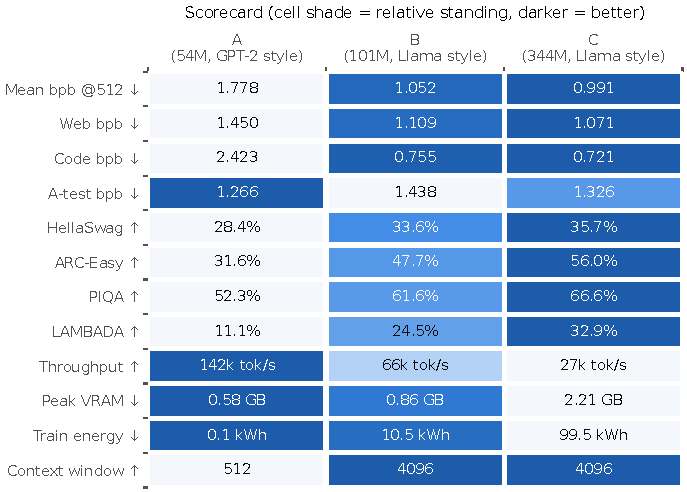
\includegraphics[width=0.62\linewidth]{figs/scorecard.pdf}
\caption{Scorecard. Each row is min--max normalised, darker = better; raw values are printed in the cells.}
\label{fig:score}
\end{figure}

\begin{table}[h]
\centering\small
\begin{tabular}{lrrr}
\toprule
Metric & A & B & C \\
\midrule
Mean bpb @512 $\downarrow$ & 1.778 & 1.052 & \textbf{0.991} \\
Web bpb $\downarrow$ & 1.450 & 1.109 & \textbf{1.071} \\
Code bpb $\downarrow$ & 2.423 & 0.755 & \textbf{0.721} \\
A-test bpb $\downarrow$ & \textbf{1.266} & 1.438 & 1.326 \\
HellaSwag $\uparrow$ & 28.4\% & 33.6\% & \textbf{35.7\%} \\
ARC-Easy $\uparrow$ & 31.6\% & 47.7\% & \textbf{56.0\%} \\
PIQA $\uparrow$ & 52.3\% & 61.6\% & \textbf{66.6\%} \\
LAMBADA $\uparrow$ & 11.1\% & 24.5\% & \textbf{32.9\%} \\
Throughput $\uparrow$ & \textbf{142k tok/s} & 66k tok/s & 27k tok/s \\
Peak VRAM $\downarrow$ & \textbf{0.58 GB} & 0.86 GB & 2.21 GB \\
Train energy $\downarrow$ & \textbf{0.1 kWh} & 10.5 kWh & 99.5 kWh \\
Context window $\uparrow$ & 512 & \textbf{4096} & 4096 \\
\bottomrule
\end{tabular}

\caption{Headline numbers (best value in bold).}
\label{tab:score}
\end{table}

\paragraph{Ranking.}
\begin{enumerate}
  \item \C{} --- best quality on every metric except A-test, the only model with reliable 4k-token context and usable math, code and chat skills. It costs the most to train, at roughly 9.5$\times$ the energy of B, and is the slowest to serve.
  \item \B{} --- the efficiency sweet spot. About 92\% of C's bpb improvement over A at 29\% of its parameters, 2.4$\times$ its throughput and a fraction of its training energy. Its weak points are long-context retrieval and LAMBADA.
  \item \A{} --- a useful educational baseline and the fastest model, but data-starved (\tppA{} tokens/param, repeated for 10 epochs), case-insensitive, limited to 512 tokens and without instruction tuning. Its quality per FLOP is the lowest of the three.
\end{enumerate}

\paragraph{Threats to validity.}
\begin{itemize}
  \item \textbf{A's lower-casing.} A predicts lower-cased, accent-stripped text while bpb is counted against the original bytes, which flatters A slightly.
  \item \textbf{Possible contamination.} B's and C's corpora come from the same sources, so B's validation shards may overlap C's training data. This would favour C on the four pipeline domains. On A-test, which neither B nor C trained on, C still beats B by about 0.11\,bpb.
  \item \textbf{Small benchmark samples.} With $n\le2000$ items, differences under about 2 points are within noise (see the intervals in Figure~\ref{fig:bench}).
  \item \textbf{Not comparable across runs.} Energy figures, and the stage results for B and C, come from each run's own logs and were not re-measured.
\end{itemize}

\FloatBarrier
\appendix
\section{Greedy samples}
{\small
\begin{longtable}{p{0.05\linewidth}p{0.05\linewidth}p{0.22\linewidth}p{0.58\linewidth}}
\caption{Greedy samples from each model ($\hookleftarrow$ marks a newline).}\label{tab:samples}\\
\toprule
Model & Mode & Prompt & Greedy continuation (64--96 tokens, truncated) \\
\midrule
\endhead
A & raw & \texttt{The capital of France is} & a french city in the province of saint-et-loire, in the province of saint-et-loire. it is located in the north of the city of saint-et-loire.    history  the capital of france was founded in the 16th century by the french gover \\
\midrule
A & raw & \texttt{Once upon a time, in a small village by the sea,} & the film is a bit slow, but the film is a bit slow, and the acting is good. the film is a little slow, but the film is a little slow, and the acting is good. the film is a little slow, but it is a little slow, and the film is a li \\
\midrule
A & raw & \texttt{def fibonacci(n):} & the supreme court on tuesday ordered the supreme court to allow the court to allow the court to allow the court to allow the court to allow the court to allow the court to allow the court to allow the court to allow the court to a \\
\midrule
A & raw & \texttt{Water boils at a temperature of} & about 2.5 degrees celsius.  the temperature of water is about 2.5 degrees celsius.  the temperature of water is about 2.5 degrees celsius.  the temperature of water is about 2.5 degrees celsius.  the temperature of water is about  \\
\midrule
B & raw & \texttt{The capital of France is} & Paris. Paris is a city known for its rich history, culture, and art. The city is known for its rich history, culture, and art. Paris is a major center for art, fashion, and fashion, and it is also a major center for art, fashion,  \\
\midrule
B & raw & \texttt{Once upon a time, in a small village by the sea,} & a woman named Luna, with a beautiful smile, stood before a man named Luna, who had been walking among the trees. Luna, with a smile, said, "Luna, I am Luna, and I am the one who brings you to this place." Luna, with a smile, \\
\midrule
B & raw & \texttt{def fibonacci(n):} &      if n <= 1:           return fibonacci(n-1)       else:           return fibonacci(n-2)     \# Driver Program   n = 10000000000000000000000000 \\
\midrule
B & raw & \texttt{Water boils at a temperature of} & 20\textdegree{}C, and then it reaches a temperature of 25\textdegree{}C. If the temperature of the water is 20\textdegree{}C, then the water boils at a temperature of 25\textdegree{}C. The total volume of water in the water is 20 + 25 = 45 liters \\
\midrule
B & chat & \texttt{Explain why the sky is blue in two sentences.} & The sky is blue in two sentences. The first sentence is about a clear, clear sky, which is a clear, clear sky. The second sentence is about a clear, clear sky, which is a clear, clear sky. The third sentence is about a clear, clea \\
\midrule
B & chat & \texttt{What is 12 * 7?} & 10 * 7 = 70; 2 * 7 = 14; 70 + 14 = 84The answer is 84. \\
\midrule
C & raw & \texttt{The capital of France is} & Paris. The current population of Paris is 271,088 in 2021. The average age of the population is 38.4 years. The standard deviation is 18.5 years.     a) What is the probability that a randomly selected person from the population \\
\midrule
C & raw & \texttt{Once upon a time, in a small village by the sea,} & there lived a kind and wise old man named Mr. Gatsby. He was known throughout the land for his love of literature and his wisdom on the subject of friendship. One day, a young girl named Lily walked into the village, curious about \\
\midrule
C & raw & \texttt{def fibonacci(n):} &      \# calculate the nth Fibonacci number      fib\_n = 0      for i in range(2, n):          fib\_n = fib\_n + fib\_n      return fib\_n    \# Driver Program   n = 10  print("Fibonacci Number", n, "is \\
\midrule
C & raw & \texttt{Water boils at a temperature of} & 100 degrees Fahrenheit and 100 degrees Celsius, respectively. If you pour water into a kettle that is at the same temperature as the kettle, how many times will the water boil before it reaches a temperature of 100 degrees Fahrenh \\
\midrule
C & chat & \texttt{Explain why the sky is blue in two sentences.} & The sky appears blue because of the way sunlight interacts with the Earth's atmosphere. When sunlight reaches the Earth's surface, it collides with molecules in the atmosphere, causing the molecules to scatter the light in all dir \\
\midrule
C & chat & \texttt{What is 12 * 7?} & 10 * 7 = 70; 2 * 7 = 14; 70 + 14 = 84The answer is 84. \\
\bottomrule
\end{longtable}

}

\section{Reproducing}
\begin{verbatim}
cd report
python3 eval_compare.py --model A --gpu 1   # also B, C  -> results/*.json
python3 gather_logs.py                      # training/energy/stage logs -> results/logs.json
python3 make_figs.py                        # figs/*.pdf, results/*.tex
latexmk -pdf report.tex
\end{verbatim}
\end{document}
